%%%%%%%%%%%%%%%%%%%%%%%%%%%%%%%%%%%%%%%%%%%%%%%%%%%%%%%%%%%%%%%%%%%%%%%%%%%
%%%                                                                     %%%
%%%   LaTeX template voor het verslag van P&O: Computerwetenschappen.   %%%
%%%                                                                     %%%
%%%   Opties:                                                           %%%
%%%     tt      Tussentijdsverslag                                      %%%
%%%     eind    Eindverslag                                             %%%
%%%                                                                     %%%
%%%   7 februari 2014                                                   %%%
%%%   Versie 1.2                                                        %%%
%%%                                                                     %%%
%%%%%%%%%%%%%%%%%%%%%%%%%%%%%%%%%%%%%%%%%%%%%%%%%%%%%%%%%%%%%%%%%%%%%%%%%%%

\documentclass[eind]{penoverslag}

%%% PACKAGES %%%
\usepackage{graphicx} 		%afbeeldingen
\usepackage{algorithmic}	%algoritmes
\usepackage{amsmath}		%wiskundige notaties
\usepackage{wasysym}		%symbolen
\usepackage{float}			%zwevende objecten
\usepackage{wrapfig}		%figuren beter weergeven
\setlength\parindent{0pt}	%geen indentatie

\begin{document}

% == TITELPAGINA == %
\team{Indigo} % teamkleur
\members{
        Wander Bavin\\
        Vince Goossens\\
        Dimitri Jonckers\\
        Sunil Tandan\\
        Wout Vekemans} % teamleden
\maketitlepage


% == SAMENVATTING == %
\begin{abstract}
\noindent
Dit rapport documenteert onze analyse en oplossing van het volgende probleem: de constructie en operatie van een zeppelin in wedstrijdverband. Navigatie gebeurt op basis van een op voorhand gekend grondplan dat wordt ingeladen in de software. De positie van de zeppelin wordt bepaald door een algoritme gebaseerd op pattern recognition. Via het rooster dient de zeppelin sneller dan een andere zeppelin naar een bepaalde positie te vliegen, daar een QR-code in te lezen en vervolgens de ingelezen opdracht uit te voeren. Beide zeppelins wisselen informatie uit met elkaar en met hun sturende pc via een server gebaseerd op RabbitMQ. Een GUI dient de toestand van het speelveld en beide zeppelins te visualiseren. Al deze functionaliteiten worden ge\"{i}mplementeerd in Java.\\
\end{abstract}


% == INHOUDSOPGAVE == %
\tableofcontents\newpage


% == INLEIDING == %
\section{Inleiding}
Dit tweede deel van de bachelorproef draait nog steeds rond het aansturen van een zeppelin op basis van een Raspberry Pi. De zeppelin moet nog steeds kunnen bewegen in de 3D-ruimte. Dit semester zal de zeppelin zich constant boven een speelveld bevinden waarop figuren liggen. Er kan dus image processing worden gebruikt om de positie exact te bepalen. De eigen zeppelin speelt een wedstrijd tegen een vijandige zeppelin van een ander team. Beiden proberen om als eerste een opgegeven bestemming te bereiken.\\
Eerst volgt er een korte beschrijving van het gebruikte materiaal en de fysieke structuur van de zeppelin. Daarna worden de uitgevoerde testen en gebruikte algoritmes beschreven. Tot slot volgt er nog een sectie die specifiek over de gebruikte en geschreven software handelt. 

\paragraph{Fysisch ontwerp}
~\\
De zeppelin bestaat uit een houten frame waaraan 2 heliumballonnen ($\diameter$90 cm) vastgemaakt zijn. Aan het frame zijn een camera en een afstandssensor vastgemaakt, die beiden naar beneden gericht zijn. Zowel de camera als de afstandssensor zijn verbonden met een Raspberry Pi die in het frame zit ingebed. Het geheel bevat drie propellers: twee voor horizontale bewegingen en \'{e}\'{e}n voor verticale bewegingen.


\paragraph{Software ontwerp}
~\\
De meeste software draait inwendig op de Pi (uitlezen sensoren, aansturen motoren, image processing). Op de sturende pc draait een GUI die de status van het speelveld weergeeft. Alle software is geschreven in Java. De communicatie tussen de zeppelins en de laptop gebeurt via een RabbitMQ server, waarlangs commando's moeten passeren die aan een vooraf afgesproken formaat voldoen. (Zie figuur \ref{schema}). \\

%% figuur van software-architectuur %%
\begin{figure}[ht!]
\centering
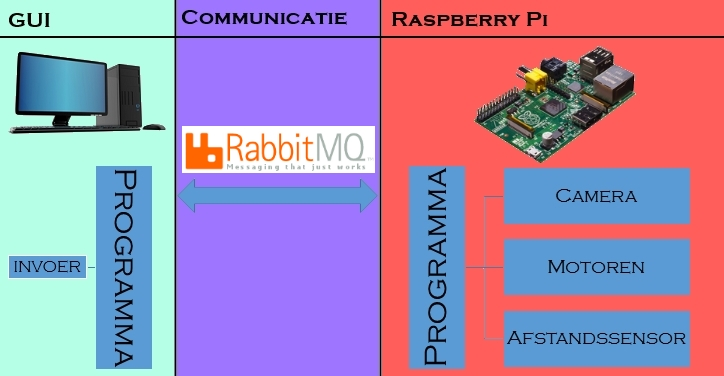
\includegraphics[height=55mm]{Schema.jpg}
\caption{Architectuur}
\label{schema}
\end{figure}

% == Beschrijving materiaal en bouw zeppelin == %
\section{Beschrijving materiaal en bouw zeppelin}
De zeppelin bestaat uit een frame waaraan alle onderdelen zijn vastgemaakt. Hierop worden onder andere de 3 motors bevestigd. Twee hiervan dienen om in het horizontale vlak te bewegen. Ze zijn met haakse draairichting op het frame (zie figuur \ref{frame}) gemonteerd. Dit staat toe om een horizontale beweging te reduceren tot een beweging in x- en y-richting, zodat het niet nodig is om te draaien (tijdens het vorige semester werd al duidelijk dat dit voor sterke afwijkingen van de zeppelin zorgt). De derde propeller dient om de zeppelin te laten stijgen, en is naar beneden gericht. De propellers kunnen op volle kracht of door middel van pwm\footnote{en.wikipedia.org/wiki/Pulse-width\_modulation} worden aangestuurd (in 2 richtingen). Met deze techniek is het mogelijk om naast de richting ook de kracht van de motor in te stellen. De onderste propeller wordt aangestuurd door de hardware-pwm op het motorbordje, terwijl voor de horizontaal gerichte propellers gebruik wordt gemaakt van SoftPWM\footnote{https://github.com/Pi4J/pi4j/blob/master/pi4j-core/src/main/java/com/pi4j/wiringpi/SoftPwm.java}. ~\\

%% figuur frame %%
\begin{figure}[h!]
\centering
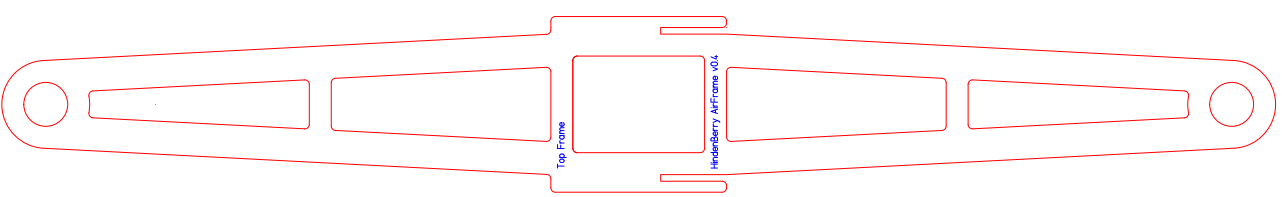
\includegraphics[scale=0.3]{upperFrame.png}
\label{frame}
\end{figure}

\begin{figure}[h!]
\centering
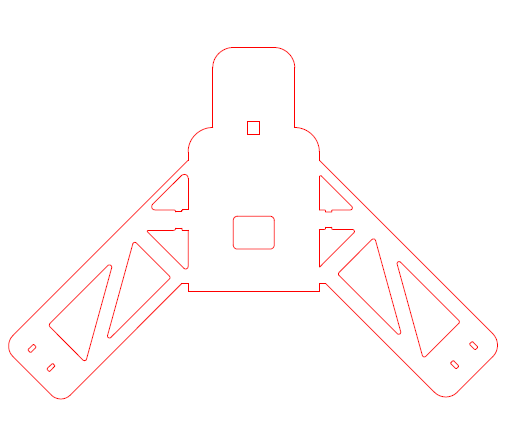
\includegraphics[scale=0.4]{lowerFrame.png}
\caption{Blueprint van het frame}
\label{frame}
\end{figure}

Voor de finale demo hebben we een nieuw frame gemaakt, dat een symmetrische gewichtsverdeling heeft als de motoren haaks op elkaar geplaatst worden. De pootjes en de ballast is behouden gebleven. Omwille van geometrische redenen (ori\"entatie van de zeppelin in xy-vlak) is de camera 45 graden gedraaid. \\

Om het geheel in de lucht te houden, zitten er 2 heliumballonnen ($\diameter$90 cm) vast aan de bovenkant van het frame. Deze hebben initieel een lift van 268 gr per stuk, maar dit vermindert wanneer de ballonnen doorheen de weken volume verliezen. \\

De zeppelin wordt aangestuurd door een Raspberry Pi model A. Deze heeft volgende specificaties:
\begin{itemize}
\item \emph{Processor:} 700MHz ARM
\item \emph{Geheugen:} 256MB
\item \emph{Poorten:} 1 USB 2.0, HDMI, audio out, RCA video
\item \emph{Voeding:} Micro USB
\item GPIO-pinnen om de hardware aan te sturen
\end{itemize}

In de Raspberry Pi zit een SD-kaart van 4 GB. Hierop staat Raspbian, het standaard besturingssysteem van de Raspberry Pi. Er is nog voldoende ruimte over om onze eigen programma's als jar-file op de Pi te zetten. \\

Verder zijn er nog 2 devices waarvan de zeppelin gebruik maakt:
\begin{itemize}
\item \emph{De camera} laat toe foto's te nemen met een maximum resolutie van 5 MP. Hij wordt in deze opdracht vooral gebruikt voor het bepalen van de positie van de zeppelin. Hiervoor neemt hij foto's van de patronen op de grond die vergeleken worden met het gekende grondplan. Daarnaast kan de camera video's maken met resoluties tot 1080p.

\item \emph{De afstandssensor} kan worden gebruikt om met ultrasone trillingen de afstand te meten tussen de zeppelin en de grond of muur. De sensor heeft een bereik van 2-400 cm. Onze afstandssensor is vooral gebruikt voor het aansturen van het hoogteregelend PID-algoritme.  \\
\end{itemize}

%% foto volledig frame
\begin{figure}[ht!]
\centering
\includegraphics[height=60mm]{FullFrame.jpg}
\caption{Frame met gemonteerde onderdelen}
\label{zeppFrame}
\end{figure}

Om het geheel te monteren, hebben we gebruik gemaakt van plakband en zipties (bundelbandjes). We hebben bekertjes bevestigd om ballast te dragen, zodat het geheel lichtjes zakt wanneer de motor geen kracht naar boven zet. Als gewicht gebruiken we zout, zodat het mogelijk is om nauwkeurig het gewicht te regelen. Tijdens het landen steunt het geheel op twee pootjes, gemaakt van piepschuimen bekertjes. \\

% == Testen == %
\section{Testen}

Om er zeker van te kunnen zijn dat het aansturen van de zeppelin correct gebeurt, is het nodig dat de componenten getest worden. In deze sectie volgt hierover meer informatie.

\subsection{Afstandssensor}
Voor gedetailleerde gegevens verwijzen we naar het verslag over onze zeppelin van het eerste semester (versie 2). Hier hadden we gemerkt dat een enkele waarde van de sensor niet noodzakelijk de correcte afstand weergeeft. Daarom houdt de afstandssensor de laatste 10 gemeten waardes bij. De huidige hoogte wordt gegeven als het gemiddelde van deze waardes (rolling median techniek). Het interval tussen twee metingen hebben we kunnen terugbrengen tot 20 ms.

\subsection{Camera en pattern recognition}
De implementatie van de pattern recognition vereist nieuwe testen van de camera om deze functionaliteit op punt te brengen. De tests proberen de verschillende moeilijkheden van de real time uitvoering te simuleren. De factoren die de positiebepaling aan de hand van de pattern recognition beinvloeden, hebben vooral betrekking tot de lichtintensiteit, de hoogte en het nemen van foto’s terwijl de zeppelin beweegt. De verschillende factoren en hun bijbehorende tests worden hieronder besproken.
\\
We hebben nog niet alle beschreven testen uitgebreid uitgevoerd.\\

\textbf{Lichtintensiteit}\\
De intensiteit van het licht be\"{i}nvloedt de detectie van de contouren en de kleuren. De belangrijkste fout bevindt zich bij de kleuren. Met behulp van een regelbare lichtbron en voldoende afschermeing van buitenaf neemt de camera foto’s van een patroon. Hierbij wordt de minimale benodigde lichtintensiteit geregistreerd en dit wordt vergeleken met de lichtintensiteit aanwezig tijdens de uitvoering. \\

\textbf{Hoogte}\\
De hoogte van de zeppelin tijdens de fotoregistratie heeft gevolgen voor het aantal vormen die geregistreerd worden en de afstand tussen de vormen op de foto. Er is een minimaal aantal vormen nodig om de positie te bepalen (3 figuren). Een succesvolle verwerking vereist een minimale hoogte, die we zullen bepalen door verschillende hoogtes te testen. Te weinig vormen op de foto zorgen ervoor dat de positie niet bepaald kan worden. Het aantal pixels tussen de verschillende contouren kan ook een negatief effect hebben op de differentiatie van de verschillende vormen. De camera neemt foto’s van een patroon van vormen gepositioneerd onder de zeppelin waarbij de hoogte steeds varieert.\\ 

\textbf{Beweging}\\
Als de zeppelin beweegt, kan dit effect hebben op de geregistreerde vormen. Een dilatie van de vormen kan plaatsvinden, waardoor bijvoorbeeld een rechthoek verandert in een ruit. Een ander mogelijk probleem constateert zich in het wazig worden van de foto’s waardoor image recognition niet met goede nauwkeurigheid plaatsvindt. Dit is belangrijk omdat het bewegen van de zeppelin tijdens het nemen van de foto dit effect kan teweegbrengen. Deze proef test het effect van de beweging, alsook de snelheid van de zeppelin op de dilatie van de figuren en de wazigheid van de foto’s.  \\

\subsection{Motoren}
In het eerste semester hebben we uitgebreide testen gedaan over de mogelijkheden van pwm. Het werd duidelijk dat het nodig ging zijn om constant de hoogte te controleren en bij te sturen. Daarnaast bleek ook dat horizontale bewegingen moeilijk exact kunnen worden uitgevoerd, omdat de zeppelin zeer gevoelig is voor allerlei veranderingen van de windomstandigheden in de omgeving: een andere zeppelin die beweegt, de airco, \ldots \\

In het tweede semester zullen we enkele testen opnieuw moeten uitvoeren, voornamelijk gerelateerd aan het gebruik van SoftPWM. Er moet bepaald worden tussen welke grenzen het vermogen groot genoeg is om de motor effectief te laten draaien. Op het moment van indienen van dit verslag zijn deze testen nog niet uitgevoerd.

% == ALGORITMES == %
\section{Algoritmes}
\subsection{Verticale bewegingen}
Om naar een bepaalde hoogte te stijgen, maken we gebruik van een PID-algoritme\footnote{http://www.csimn.com/CSI\_pages/PIDforDummies.html}. Hierbij gaan we op basis van de huidige fout in hoogte, bepalen of de zeppelin moet stijgen of dalen en met welke kracht. Daarnaast wordt rekening gehouden met de afgeleide, om toekomstige veranderingen te voorspellen. Tenslotte is er de integraal, die fouten uit het verleden voorstelt. Op basis hiervan wordt een pwm-waarde voor de motor gegeven. Het algoritme wordt aangepast aan het gewicht van onze zeppelin en de kracht van de gegeven motoren. Dit gebeurt door middel van trial-and-error om de constanten van de regelaar te bepalen.\\
De output wordt berekend op basis van deze formule:

\begin{center}
$output = Kp*error + Ki*integral + Kd*derivative$\\
\end{center}

Hierin zijn Kp, Ki en Kd constanten die we hebben moeten bepalen. Eerst hadden we enkel rekening gehouden met de huidige error (Ki = Kd = 0), maar dit bleek er voor te zorgen dat de zeppelin veel te snel naar een bepaalde hoogte gaat en er dan ver boven of onder gaat. We hebben dit opgelost door Kd te verhogen. Door deze groot te maken, gaat de zeppelin veel rustiger naar de opgegeven hoogte en gaat hij er niet voorbij. Bij de start van het tweede semester hebben we de waardes van deze constanten opnieuw getuned, aangezien er nieuwe volle ballonnen gegeven waren. \\

Er is een HeightController die dit PID-algoritme implementeert, en die er voor gaat zorgen dat de zeppelin zijn hoogte behoudt of naar een gevraagde hoogte gaat. Deze gaat om de 0.1 s de hoogte controleren en de pwm-waarde bijsturen. \\

\subsection{Horizontale bewegingen}
Voor bewegingen in het horizontale vlak maken we eveneens gebruik van PID-gebaseerde algoritmes. We gebruiken twee afzonderlijke algoritmes die tegelijk lopen (voor de x- en y-richting). Telkens wanneer een nieuwe foto genomen wordt, kunnen we hieruit de positie en draaiing ten opzichte van het veld afleiden. Dan kunnen we de af te leggen afstand ontbinden in twee loodrechte bewegingen (x- en y-richting ten opzichte van het veld). De zeppelin wordt in het middelpunt geplaatst van het nieuwe co\"{o}rdinatenstelsel. De co\"{o}rdinaten van de bestemming in het geroteerde en verschoven assenstelsel bepalen dus exact hoeveel we in x- en y-richting moeten bewegen. De omzetting gebeurt in 2 stappen, met eerst een verschuiving:\\
\centerline{$x_{shifted} = x_{destination} – x_{zeppelin}, y_{shifted} = y_{destination} – y_{zeppelin}$}\\

Vervolgens doen we een draaiing volgens de hoek $\alpha$ waarmee de zeppelin gedraaid staat ten opzichte van het frame:\\
\centerline{$x_{new} = x_{shifted}*cos(\alpha) + y_{shifted}*sin(\alpha)$}\\
\centerline{$y_{new} = -x_{shifted}*sin(\alpha) + y_{shifted}*cos(\alpha)$}\\

Nu geven we deze nieuwe x- en y-waarden als bestemming door aan de bijbehorende PositionController, zodat de PID-regelaar de juiste motor bijstuurt. Zie verder voor het UML-schema met de klassen die gebruikt worden voor horizontale navigatie (figuur \ref{navigation}).



\subsection{Pattern recognition}
De camera neemt foto’s van de patronen op het veld onder de zeppelin. De Raspberry Pi bewerkt deze foto’s met behulp van zelfgeschreven software. Op elk geregistreerd beeld wordt dezelfde sequentie van operaties uitgevoerd. \\
Als eerste herkent de software de simpele vormen. De functionaliteit van het programma beperkt zich tot de mogelijke vormen meegedeeld in de probleemstelling (cirkel, rechthoek, vijfpuntige ster, hart).Een omvorming naar zwart-wit vergemakkelijkt dit. De vormherkenningalgoritmes (pattern recognition) registreren de contouren van de vormen en halen de nuttige contouren uit het waargenomen beeld. Operaties in het algoritme verwijderen contouren die geen betrekking hebben tot de vormen. Vervolgens benadert de software de overgebleven contouren door polygonen (veelhoeken). Op basis van de punten van deze benaderingen en kenmerken van de mogelijke vormen haalt het algoritme de corresponderende vorm(en) uit de foto. Bijvoorbeeld: De punten op een cirkel bevinden zich op een vaste afstand van het middelpunt, de lengte van een rechthoek is gelijk aan de gesommeerde afstand tussen de de vier hoekpunten,\ldots \\
Eenmaal de vorm gespecificieerd is, dient de kleur nog bepaald te worden.  Het programma converteert hiervoor de foto naar een HSV-digitale voorstelling. De minimale en maximale waarden voor respectievelijk H,S en V, die karakteristiek zijn voor de mogelijke kleuren, bepalen de aanwezige kleur binnen de contour van de gedetecteerde vorm. Voor een visualisatie van de verschillende stappen, zie figuur \ref{Patterns}. \\

Hierbij dient wel vermeld te worden dat de pattern recognition nog niet volledig werkt. Het werken met OpenCV in Java bracht heel wat problemen met zich mee. Op het moment van het schrijven van dit verslag lukt het in de meeste afbeeldingen om figuren te herkennen (maar nog niet het hart en de ster). Dit werkt echter enkel nog maar op de pc, aangezien het installeren van OpenCV die werkt met Java op de Pi nog problemen oplevert. Verder hebben we ook nog niet veel getest met het herkennen van images die genomen zijn terwijl de zeppelin beweegt.

\begin{figure}[H]
\begin{center}
\includegraphics[width=0.8\textwidth]{patternrecognition.png}
\end{center}
\caption{Pattern Recognition}
\label{Patterns}
\end{figure}

\subsection{Locatiebepaling}
Om de locatie te bepalen wordt er gebruik gemaakt van een set van symbolen. Deze zijn in het ideale geval herkend door het pattern recognition algorithm. Elk symbool heeft een kleur en vorm en een x- en y-coördinaat binnen de afbeelding. Eerst bepaalt het algoritme (zie verder) welk van de gegeven symbolen het meest centraal ligt ten opzichte van de andere symbolen. Dit symbool wordt het middelpunt.\\

Vervolgens zoekt het algoritme driehoeken. Een driehoek bestaat uit het middelpunt en twee punten die op de kortst mogelijke afstand van elkaar liggen. Een driehoek bepaalt eenduidig de locatie van de zeppelin omdat elke driehoek maar \'e\'en keer mag voorkomen. Om driehoeken te detecteren kijken we welke punt er het dichtst bij het middelpunt ligt, en filteren we de andere punten zodat we enkel punten overhouden waarvoor de afstand tot het middelpunt binnen een bepaalde marge ligt (1.2x kortste afstand). Deze punten worden gesorteerd op poolcoördinaten. Vervolgens selecteren we twee punten die samen met het middelpunt een driehoek vormen. Deze twee punten mogen wel maximum 1,2x de kortste afstand uit elkaar liggen (voor het geval er symbolen ontbreken) en het tweede punt moet in wijzerzin van het eerste punt liggen.\\

Dan kan het echte vergelijken met het raster gebeuren: alle punten van het veld worden afgegaan. Indien het middelpunt overeen komt met een punt uit het raster, worden alle buren van dit punt opgevraagd. Indien de andere twee punten van de gevonden overeen komen met twee buren, die ook naast elkaar liggen en in dezelfde volgorde staan, hebben we een match en hebben we de locatie gevonden. De locatie die wordt teruggegeven is de locatie van het middelpunt.\\

\textbf{Locate: }
\begin{algorithmic}

	\STATE in: Symbols; out: location
	\STATE Symbol center = calculateCenter(symbols)
	\STATE Symbol closestToMid = closestSymbol(symbols,center)     //get symbol closest to center symbol
	\STATE closestToMidDist = dist(center,closestToMid)
	\STATE List $\textless$Symbol$\textgreater$ neighbours = filter(symbols,1.2*closestToMidDist)
	\STATE neighbours = sortPolar(neighbours,center)     //sort around center
	\FOR {Symbol s1 in neighbours}
		\STATE s2 = next(s1) %symbol following s1
		\IF{dist(s1,s2) $\le$ 1.2*closestToMidDist \&\& clockwise(s1,s2)}
			\STATE location = match(center,s1,s2)
		\ENDIF
	\ENDFOR
	
\end{algorithmic}

\textbf{Match:}
\begin{algorithmic}
\STATE In: center, s1, s2; out: location, rotation
	\FOR{Symbol s on map}
		\IF{s matches center}
			\FOR{Symbol sm1 in map.neighbours(center)} 
				\STATE sm2 = next(sm1)
				\IF{s1 matches sm1 \&\& s2 matches sm2}
					\STATE location found
					\STATE calculate $\alpha$
					\STATE return location, $\alpha$
				\ENDIF
			\ENDFOR
		\ENDIF
	\ENDFOR
\end{algorithmic}




% == SOFTWARE == %
\section{Software}

Alle software voor dit project is in Java geschreven. Deze keuze is tijdens het eerste semester al gemaakt omdat dit voor het hele team de gebruikte programmeertaal was, en omdat er voldoende voorbeeldcode te vinden was om te programmeren op de Pi. We hebben in het eerste semester ook geen problemen gehad met het implementeren van functionaliteit in Java (aansturen motoren, QR-codes). Dit semester zijn we wel op veel moeilijkheden gestoten bij het implementeren van image recognition. \\
Een andere oplossing, door veel concurrenten gekozen, is Python. Een nadeel hiervan is dat iedereen dan een nieuwe taal zou moeten leren, wat het ontwerpproces enorm vertraagt. Het voordeel is wel dat Python makkelijker is om te werken met de Raspberry Pi. \\ 

Een gedeelte van de code is overgenomen van ons project van vorig semester. Deze is echter volledig opgefrist, waardoor de code veel overzichtelijker is geworden. Stukken software die toen door tijdsgebrek ergens werden bijgezet, zijn verplaatst naar waar ze echt thuishoren. Enkele basiselementen zoals het aansturen van de motoren zijn echter hetzelfde gebleven.\\

\subsection{GUI}
De GUI stelt de gebruiker in staat om vanaf een pc verbinding te maken met de RabbitMQ-server die het speelveld en de zeppelins controleert. De GUI geeft dan informatie weer over het speelveld, de co\"{o}rdinaten van de zeppelins, en de bestemming. \\

%GUI afbeelding %
\begin{figure}[H]
\begin{center}
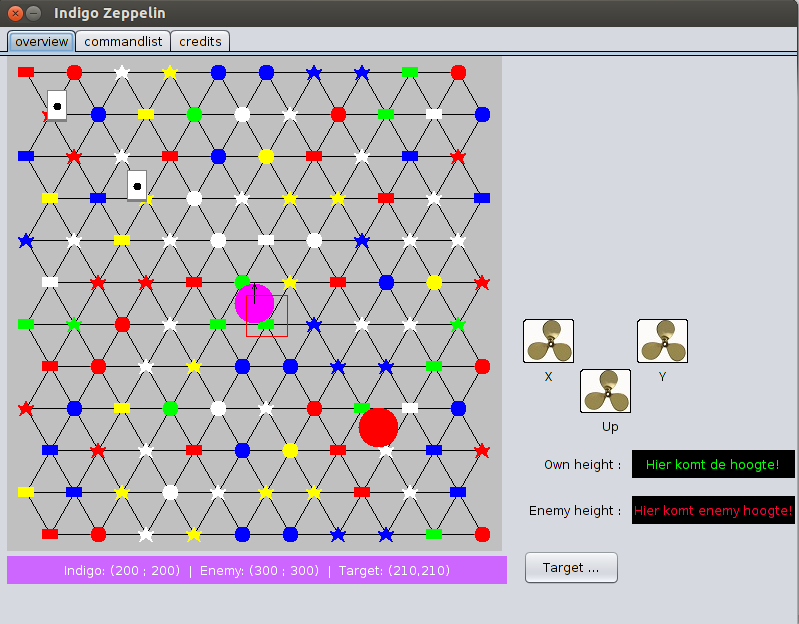
\includegraphics[width=0.6\textwidth]{GUI.png}
\end{center}
\caption{GUI}
\label{GUI}
\end{figure}

De eerste tab (`overview') toont de hoogte van beide zeppelins, alsook de toestand van de eigen propellers. Een kaart geeft de locaties van de zeppelins weer. De kaart wordt uitgelezen (zoals al beschreven bij het algoritme voor plaatsbepaling) en omgezet naar een afbeelding. Op de afbeelding verschijnen ook de posities van de eigen zeppelin en de vijandige zeppelin, en de bestemming. Naast de kaart wordt de opdracht van de zeppelins getoond en is er een overzicht van de laatste berichten die zijn uitgewisseld tussen de pc en de zeppelin. \\

De tweede tab geeft een uitgebreider overzicht van alle informatie die wordt uitgewisseld tussen server, GUI en zeppelin, met een tijdsindicatie. Er is de mogelijkheid om berichten te filteren op type. \\

\subsection{Pattern recognition, locatiebepaling en horizontale beweging}
De eerder vermelde pattern recognition is gemaakt met behulp van de Java-library OpenCV\footnote{http://opencv.org/}. Hiermee kan detectie van vormen en kleuren worden ge\"{i}mplementeerd. Het is de bedoeling dat de image recognition zelf op de Pi gebeurt, maar op dit moment hebben we enkel nog maar kunnen testen met het verwerken van afbeeldingen op een pc. Hieronder is een klassediagram te vinden waarop de belangrijkste klasses voor pattern recognition zichtbaar zijn.\\
De motorcontroller gaat op geregelde tijdstippen een foto nemen via de camera. Deze wordt dan omgezet naar een lijst van figuren door de ImageProcessor. De LocationLocator kan hieruit de huidige positie van de zeppelin bepalen. Nu gaat de PositionController de af te leggen afstand in x- en y-richting bepalen. Beide richtingen hebben een Controller, die met een PID-algoritme de respectievelijke motoren aansturen.\\

%Klassendiagram Bewegingen
\begin{figure}[H]
\begin{center}
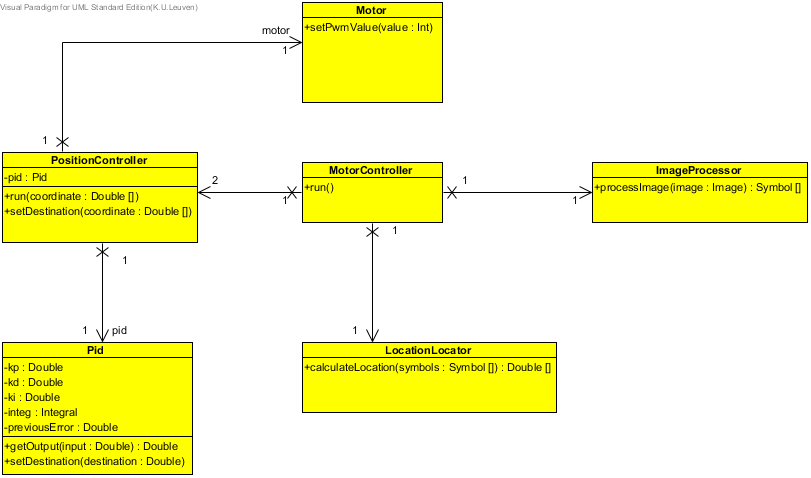
\includegraphics[width=\textwidth]{XYNavigation.png}
\end{center}
\caption{UML-schema horizontale bewegingen}
\label{navigation}
\end{figure}

\subsection{Connectie}
De verbinding tussen Pi en laptop is volledig veranderd. Voordien werd informatie uitgewisseld door middel van sockets, op een virtueel netwerk gehost vanuit een laptop. Communicatie verliep via sockets over dit netwerk. De Pi werd toen de server genoemd omdat deze de sockets initialiseerde. Deze opdracht verplicht ons gebruik te maken van een RabbitMQ server\footnote{www.rabbitmq.com}. Voor de eerste tussentijdse demo zal de server op een eigen laptop worden gestart, omdat er geen communicatie met een andere zeppelin nodig is. We hebben nu dus de server (de exchange) die losstaat van de rest van het programma, en twee clients: de zeppelin (Pi) en de GUI. Zowel GUI als Pi connecteren dan op een exchange genaamd ‘server’. Elke boodschap die wordt uitgewisseld krijgt een bepaalde sleutel toegewezen, die aangeeft wat de boodschap bevat en voor wie ze bestemd is. Een boodschap wordt dan naar de exchange verstuurd. De exchange weet dankzij de sleutel naar welke queue hij de boodschappen moet versturen. Zowel de GUI als de Pi abonneren zich op queues met een bepaalde sleutel, afhangende van welke gesleutelde boodschappen ze willen ontvangen. Om gebruik te maken van rabbitMQ in onze code moesten er enkele libraries\footnote{http://www.rabbitmq.com/java-client.html} toegevoegd worden. Het sequentiediagram (zie figuur \ref{Sequence}) is te zien hoe een low-levelopdracht voor het aanschakelen van de motoren aan een bepaalde snelheid wordt doorgegeven vanaf een client naar de Pi. Vanuit de GUI wordt er steeds via de klasse GUICommands gegaan, die een abstractie geeft naar buiten toe. Klasses voor communicatie versturen en ontvangen de boodschap (met toevoeging van correcte sleutel) via RabbitMQ. De MotorController gaat uiteindelijk bepalen dat de x-motor aan een bepaalde SoftPwm-value moet draaien.
\\

%Sequentiediagram communication Pi Client
\begin{figure}[H]
\begin{center}
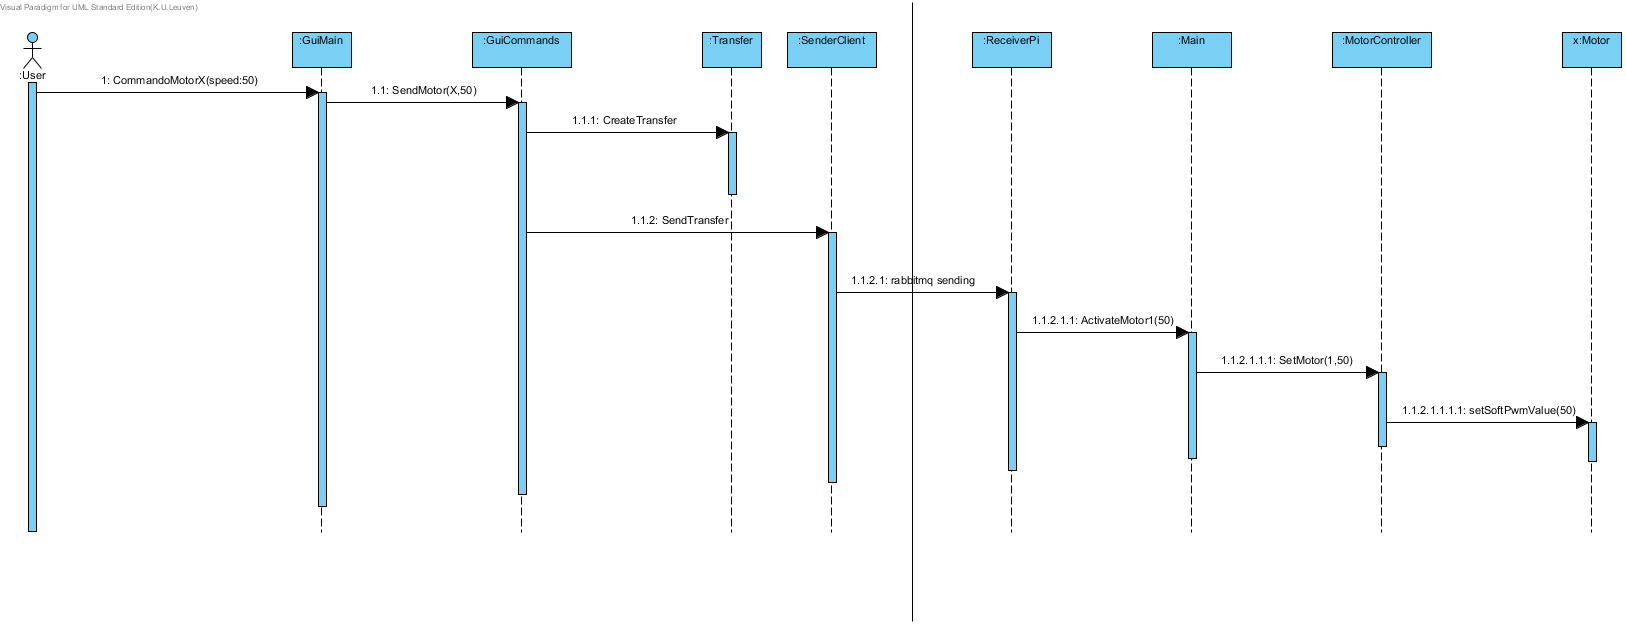
\includegraphics[width=1\textwidth]{PiToClientCommunication.png}
\end{center}
\caption{Sequentiediagram van de communicatie}
\label{Sequence}
\end{figure}

\subsection{Simulator}
Naar de toekomst toe zijn we van plan een simulator te maken, die de toestand van het spel simuleert. Dit stelt ons in staat om algoritmes (bijvoorbeeld om een tegenstander te ontwijken) uit te testen zonder dat we echt met twee zeppelins op het speelveld moeten zitten.\\
Momenteel is deze nog niet geschreven, maar het plan is dat deze een kaart maakt of een gegeven kaart gebruikt, en hierop een bestemming kiest. De image processing zal worden uitgeschakeld, en de zeppelin zal een reeks symbolen krijgen van de simulator die normaal door de image processing herkend zouden zijn. Voor de rest gaat de zeppelin zich gedragen zoals ook in realiteit het geval is: de informatie over de symbolen binnenkrijgen, hieruit zijn plaats bepalen, en zijn positie bijsturen. Deze moet dan worden doorgegeven aan de simulator in plaats van aan de motoren. We zijn ook van plan om een optie toe te voegen die op geregelde tijdstippen een afwijking op de beweging zet, omdat dit iets is wat in realiteit ook onvermijdelijk zal gebeuren.\\
De stukken van de zeppelin die we hiervoor dynamisch gaan moeten wijzigen zijn de input van herkende symbolen, en de output naar simulator in plaats van motoren van de PositionController.


% == BESLUIT == %
\section{Besluit}
De uitvoering van de toevoegingen aan soft- en hardware zijn vrij goed gelukt. We zijn tevreden over de kwaliteit van de code, die nu veel ordelijker is dan vorig semester. Het implementeren van pattern recognition en de bijhorende navigatie brachten wel enkele moeilijkheden met zich mee. Het communiceren met een RabbitMQ-server hadden we vrij snel onder de knie en dit bracht slechts kleine aanpassingen met zich mee. Het probleem op dit moment is de navigatie en positieherkenning. De navigatie op zich zou kunnen werken, maar hiervoor is positieherkenning nodig en moet dus de image processing goed werken. \\
We hebben een nieuw frame ontworpen dat het besturen van de zeppelin zou moeten vergemakkelijken.
%insert hier nog iets over hoe het effectief werkt aangezien we nog nie hebben gevlogen %
Naar de demo toe gaan we nog zoveel mogelijk proberen te testen op het herkennen van images en op vliegen. \\
Naar de volgende demo toe zal de software moeten uitgebreid moeten worden om volledig aan het afgesproken protocol voor communicatie te voldoen en om te zorgen dat de zeppelin Ook moeten we de zeppelin in contact brengen met een andere zeppelin. \\

% == APPENDICES == %
\newpage\makeappendix

\section{Beschrijving van het proces}
Dit onderdeel maakt geen deel uit van dit verslag.


\section{Beschrijving van de werkverdeling}
Een overzicht van de taken van de groepsleden: \\
\begin{itemize}
\item Wander Bavin: Vervulde de rol van co\"ordinator en van vertegenwoordiger in de scheidsrechtercommissie. Hiervoor heeft hij zich beziggehouden met onderzoek van RabbitMQ, met het schrijven van een deel van de software voor de server, en met voorstellen voor een protocol voor de voorstelling van commando's. Hij heeft ook het gedeelte van de communicatie verzorgt, en in het begin even meegewerkt aan de nieuwe GUI. Heeft zich ook beziggehouden met het opruimen van code van het eerste semester en het maken van UML-diagrammen.
\item Dimitri Jonckers: Heeft de GUI herschreven en zich beziggehouden met het opruimen van code van het eerste semester. Heeft gewerkt aan het verslag en de UML-diagrammen. Heeft een deel van de nieuwe code voor de zeppelin geschreven (positiecontrole, bewegingsalgoritme). Verder heeft hij het uitlezen van de map verzorgt.
\item Sunil Tandan: Heeft zich grotendeels beziggehouden met onderzoek naar pattern recognition en hier software voor geschreven. Verder heeft hij gewerkt aan een algoritme voor het bepalen van de plaats op basis van de figuren.
\item Wout Vekemans: Vervulde de rol van secretaris. Heeft zich voor een groot stuk beziggehouden met het verslag. Heeft een deel van de nieuwe code voor de zeppelin geschreven (positiecontrole). Hij ligt ook mee aan de basis van de nieuwe GUI. In het tweede deel van het semester heeft hij het nieuwe frame ontworpen en gemonteerd. 
\item Vince Goossens: Heeft zich grotendeels beziggehouden met onderzoek naar pattern recognition en hier software voor geschreven. Verder heeft hij gewerkt aan een algoritme voor het bepalen van de plaats op basis van de figuren.
\end{itemize}

Hieronder is een tabel te vinden met de gewerkte uren binnen en buiten de sessies: \\

\begin{tabular}{r||r|r|r|r|r}
Overzicht: & Dimitri Jonckers & Wander Bavin & Wout Vekemans & Sunil Tandan & Vince Goossens \\
\hline \hline
10/02 - 16/02 & 9 & 12.5 & 7 & 11 & 9 \\
17/02 - 23/02 & 17.5 & 16.5 & 7.5 & 7.5 & 11 \\
24/02 - 02/03 & 15 & 6 & 9.5 & 18.5 & 9.25 \\
03/02 - 05/02 & 6 & 5 & 8 & 9 & 9 \\
\hline \hline
Totaal & 47.5 & 40 & 32 & 46 & 38.25 \\
\end{tabular}


\section{Kritische analyse}
Dit onderdeel maakt geen deel uit van dit verslag.


\end{document}
